	\section{Domainmodel} 
		\subsection{Domain}
		
			\subsubsection{Verknüpfungen von Task Vorlagen und Entscheidungen oder Entscheiden}			
				Entscheidungen und Entscheiden werden Task Vorlagen zugeordnet. Aus diesen Vorlagen werden beim Export Tasks generiert. Taskvorlagen sind generisch, sodass Änderungen auch alle verknüpften Entscheide und Entscheidungen betreffen sollten. Aus diesem Grund werden Task Vorlagen bei der Zuordnung verknüpft und nicht kopiert.
				
				\begin{figure}[H]
					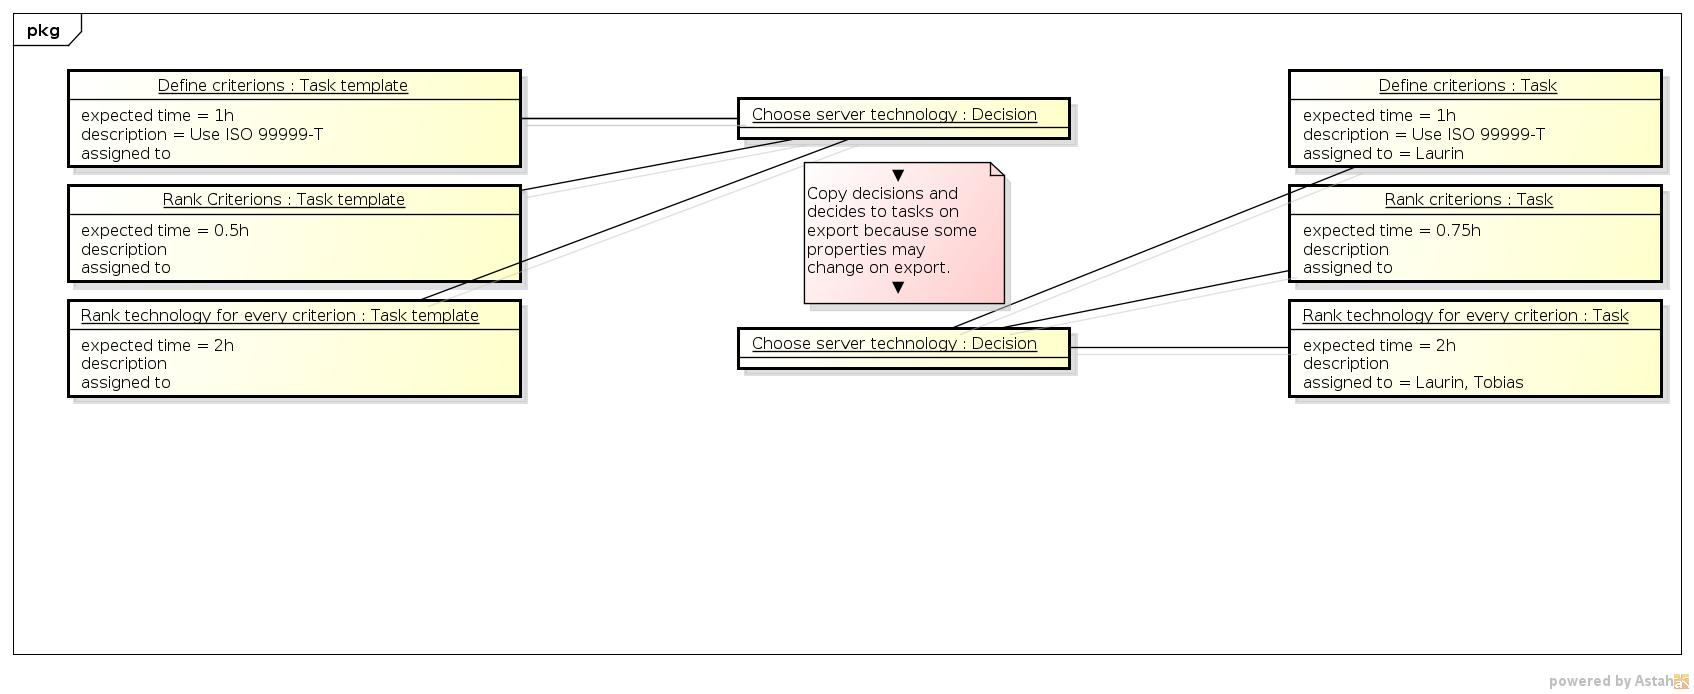
\includegraphics[width=\textwidth]{architecture/media/img/DecisionTaskRelation.jpg}
					\centering
					\caption{Exportieren von Entscheidungen und Entscheiden}
					\label{fig:DecisionTaskRelation}
				\end{figure}
				
				Beim Exporten werden aus Taskvorlagen konkrete Tasks. Auch Entscheidungen und Entscheide werden zu Tasks. Verknüpfte Tasks werden somit zu sub-tasks.
				
				Benutzer wollen beim Export die von der Task Vorlage vorgegebenen Werte möglicherweise anpassen, wie z.B. den erwarteten Aufwand für den Task.

				Daher ist es sinnvoll, die Eigenschaften der Taskvorlagen in die konkreten Tasks zu kopieren, anstatt sie lediglich zu verknüpfen.
				
				Gleiches gilt für Entscheidungen und Entscheide. Würde jemand im CDAR diese verändern oder Löschen, so würde dies die History zerstören.
				
			
			\subsubsection{EEPPI Domain}
			
				
		
		\subsection{Communication}